\section{Results}\label{sec:results}

In this section, we overview the performance results and the resource
utilization all the kernels implemented on GPU for face detection. 
Although, occupancy is not a direct measure of performance, it is important 
to have full occupancy for the GPU SMs. Based on the utilization analysis done for all the kernels,

Table~\ref{table:util} shows the occupancy of each of the kernels. This includes the registers, 
shared memory and constant memory used for the kernels. As discussed in Section~\ref{sec:haar_optim}, 
relaxing the maximum registers used by thread is an optimization. We apply this optimization and check for the 
occupancy of each kernel. 
However, this constraint can be relaxed only if all the threads in the thread block can accommodated with that register usage.
In our case, relaxing this constraint did not put a constraint on the threads that can be launched with each kernel.
We see that for \emph{RowScan Only} kernel the occupancy reduces due to this relaxation. However, the results of that kernel
show that it did not impact for the performance. 


\begin{figure*}
  \centering
  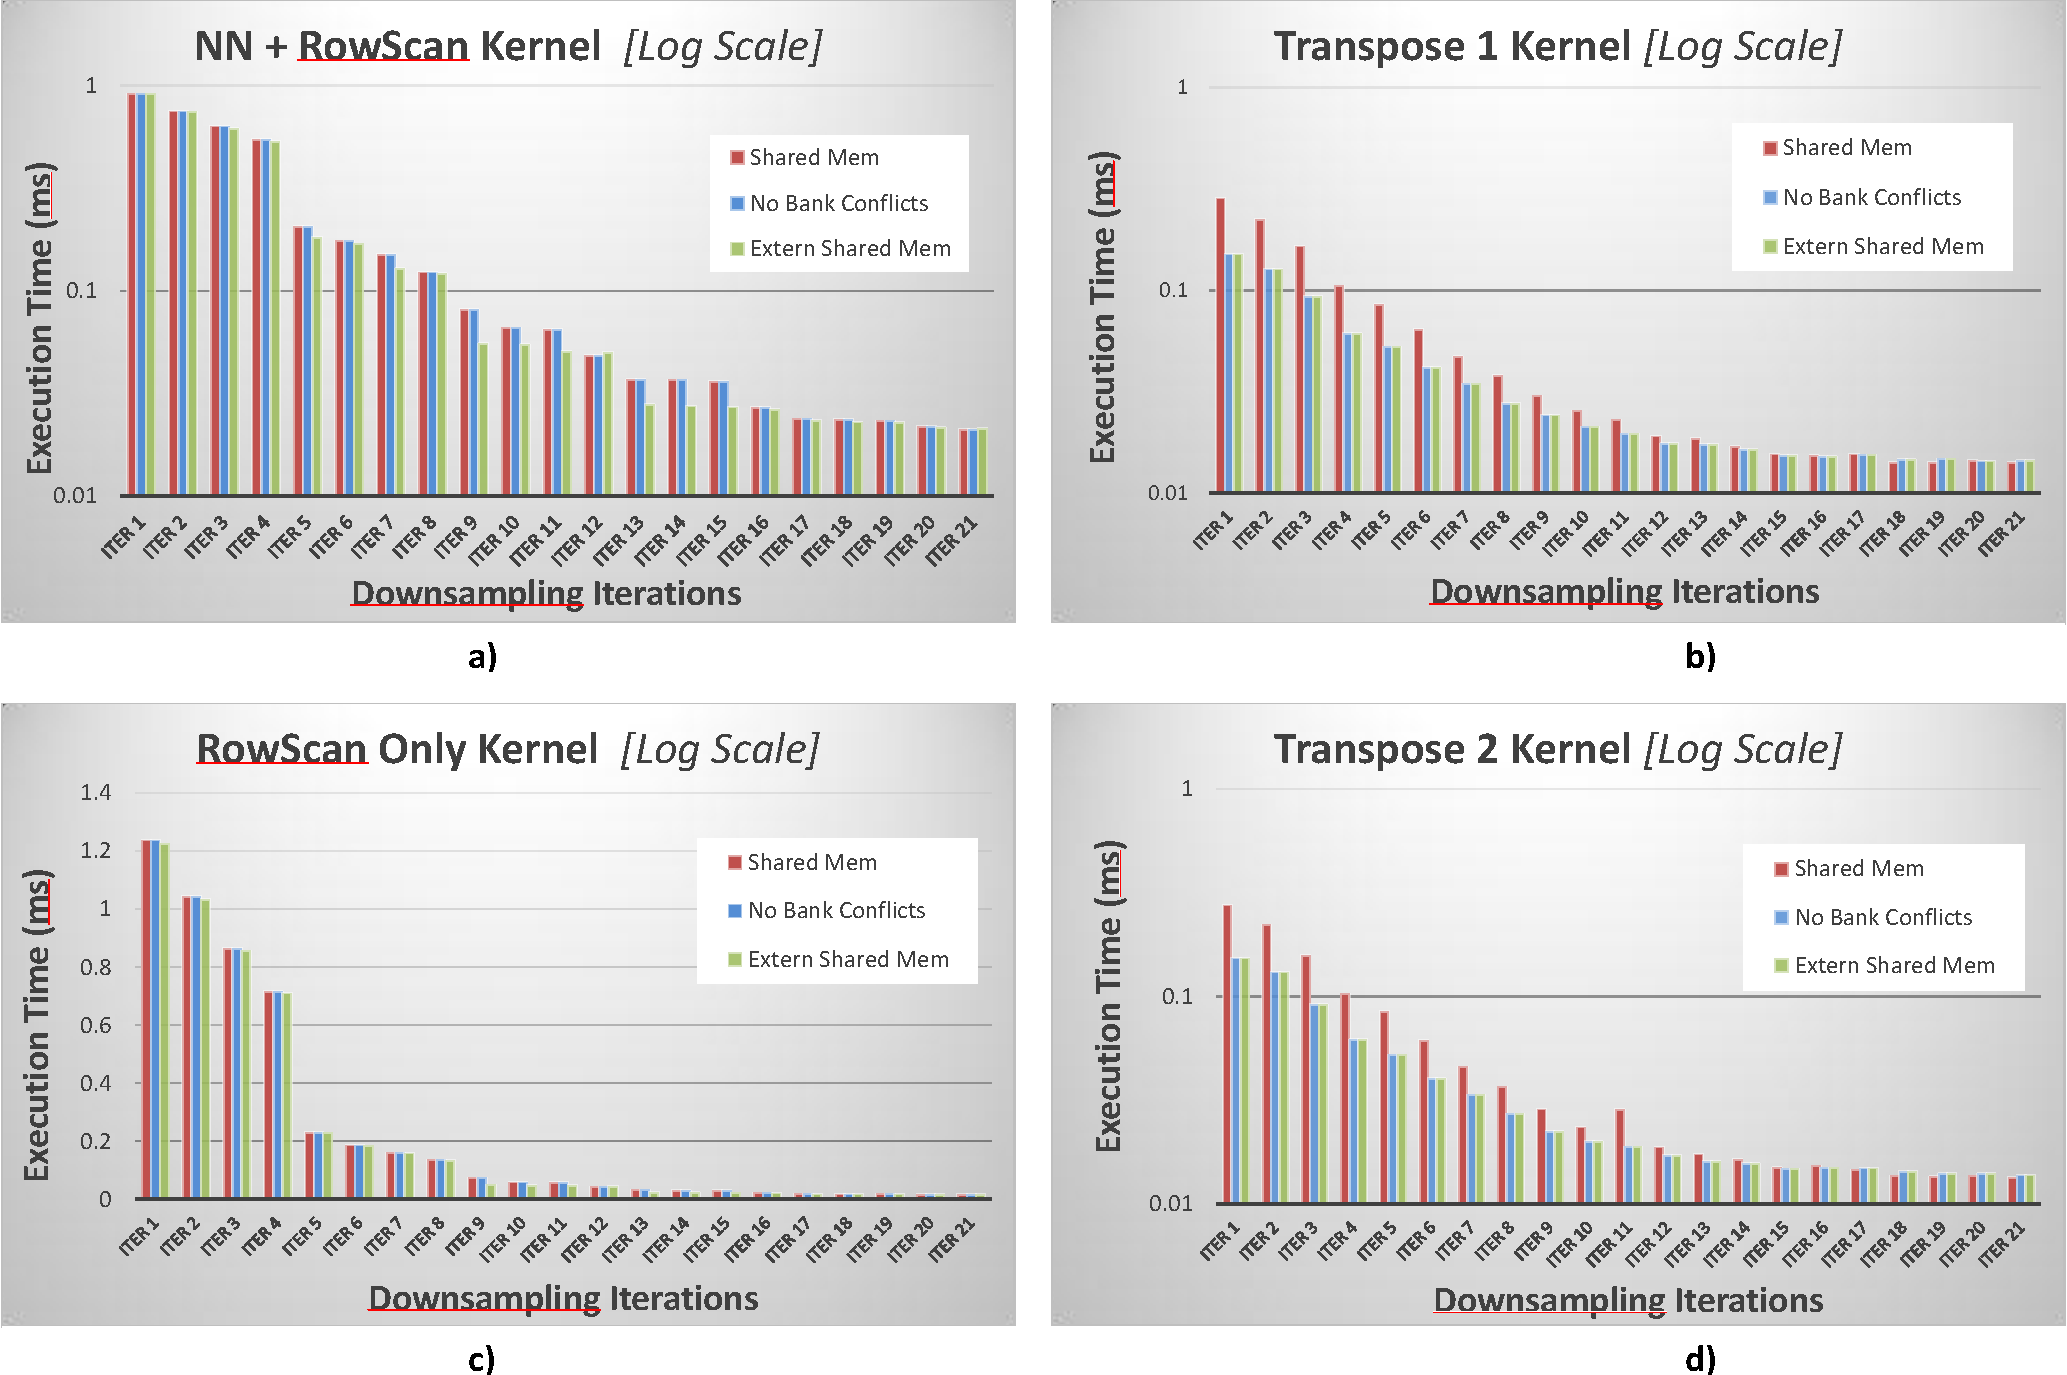
\includegraphics[width=\linewidth]{figs/nn_ii_kernels_crop.pdf}
  \caption{Performance of NN and II kernels; a) NN + RowScan; b) Transpose 1; c) RowScan Only; d) Transpose 2}
  \label{fig:nn_ii_kernels}
\end{figure*}

\vspace{0.2in}
\begin{figure*}[h]
  \centering
  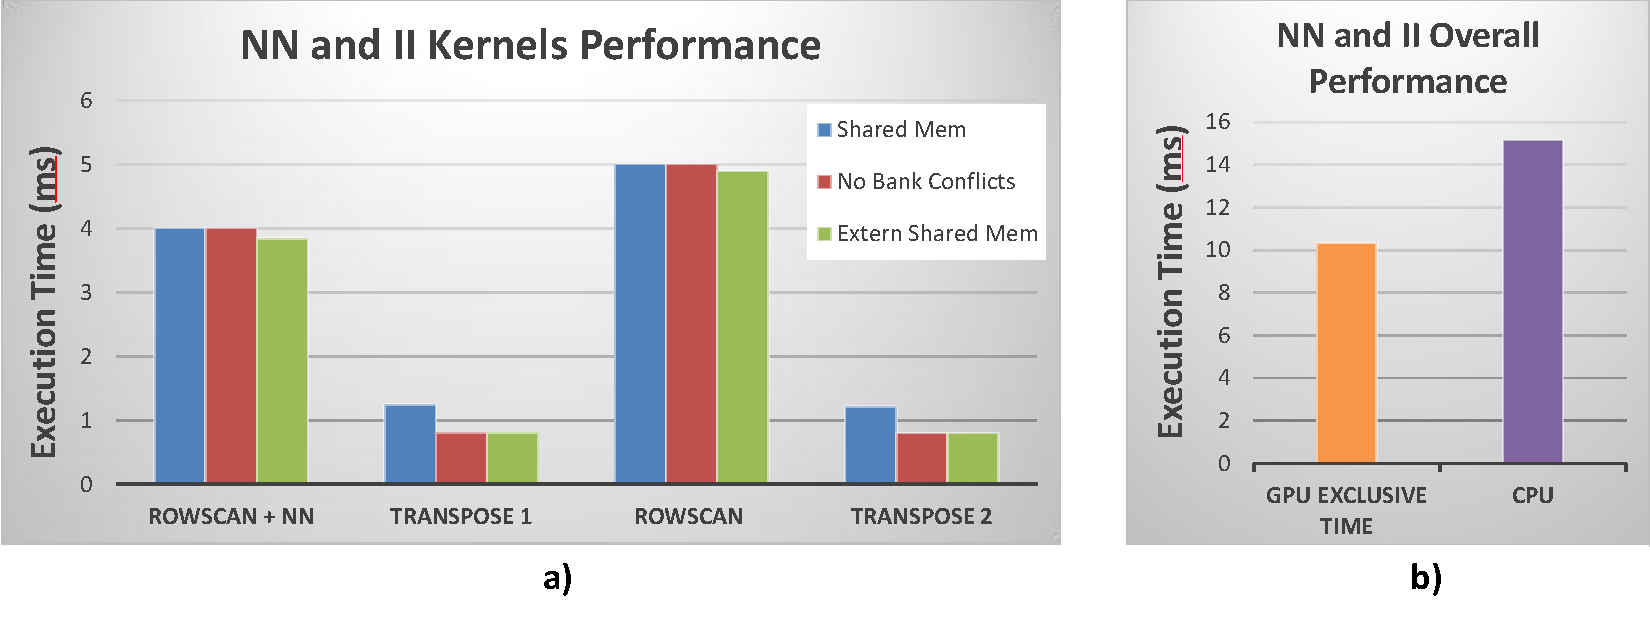
\includegraphics[width=0.9\linewidth]{figs/nn_ii_overall_crop.pdf}
  \caption{a) NN and II kernels performance for all optimizations; b) Overall NN + II performance over CPU}
  \label{fig:nn_ii_overall}
\end{figure*}

\subsection{Performance of Nearest Neighbor and Integral Image Kernels}
Figure~\ref{fig:nn_ii_kernels} shows the performance of individual kernels of NN and II stage.
We apply the 3 optimizations discussed in Section~\ref{sec:nn_optim} here. Since, NN and II kernels 
contributed to only 3\% of the overall parallelization scope, we directly implemented the Shared memory version of the kernels
and that act as the baseline for NN and II kernels. When we applied the \emph{No bank conflicts} optimization, only the \emph{Transpose 1}
and \emph{Transpose 2} kernel showed the benefit in reducing the execution time. This is because, transpose kernels are tiled implementations, 
and are initially brought from global memory to shared memory (by reading row wise) and are then read column wise from shared memory. While reading column wise, 
you encounter bank conflicts and to reduce this, we applied \emph{No bank conflicts} optimization. \emph{NN + RowScan} and \emph{RowScan} kernels do not show 
any improvement as they do not suffer from bank conflicts. 

Second optimization we applied was the external declaration of shared memory
to reduce the shared memory constraint on thread blocks and thus performance. Here in this case,
\emph{NN + RowScan} and \emph{RowScan} kernels show benefit after iteration 9 at which the size of the 
downsampled image is 256 x 256. At this scale of image, external declaring the shared memory reduced the 
pressure on shared memory usage and more thread blocks could be launched. However, \emph{Transpose 1 } and 
\emph{Transpose 2} kernels do not show any benefit as they are tiled implementation and have fixed 16 x 16 thread block
size across all the downsampled image sizes. 


\begin{figure*}[h]
  \centering
  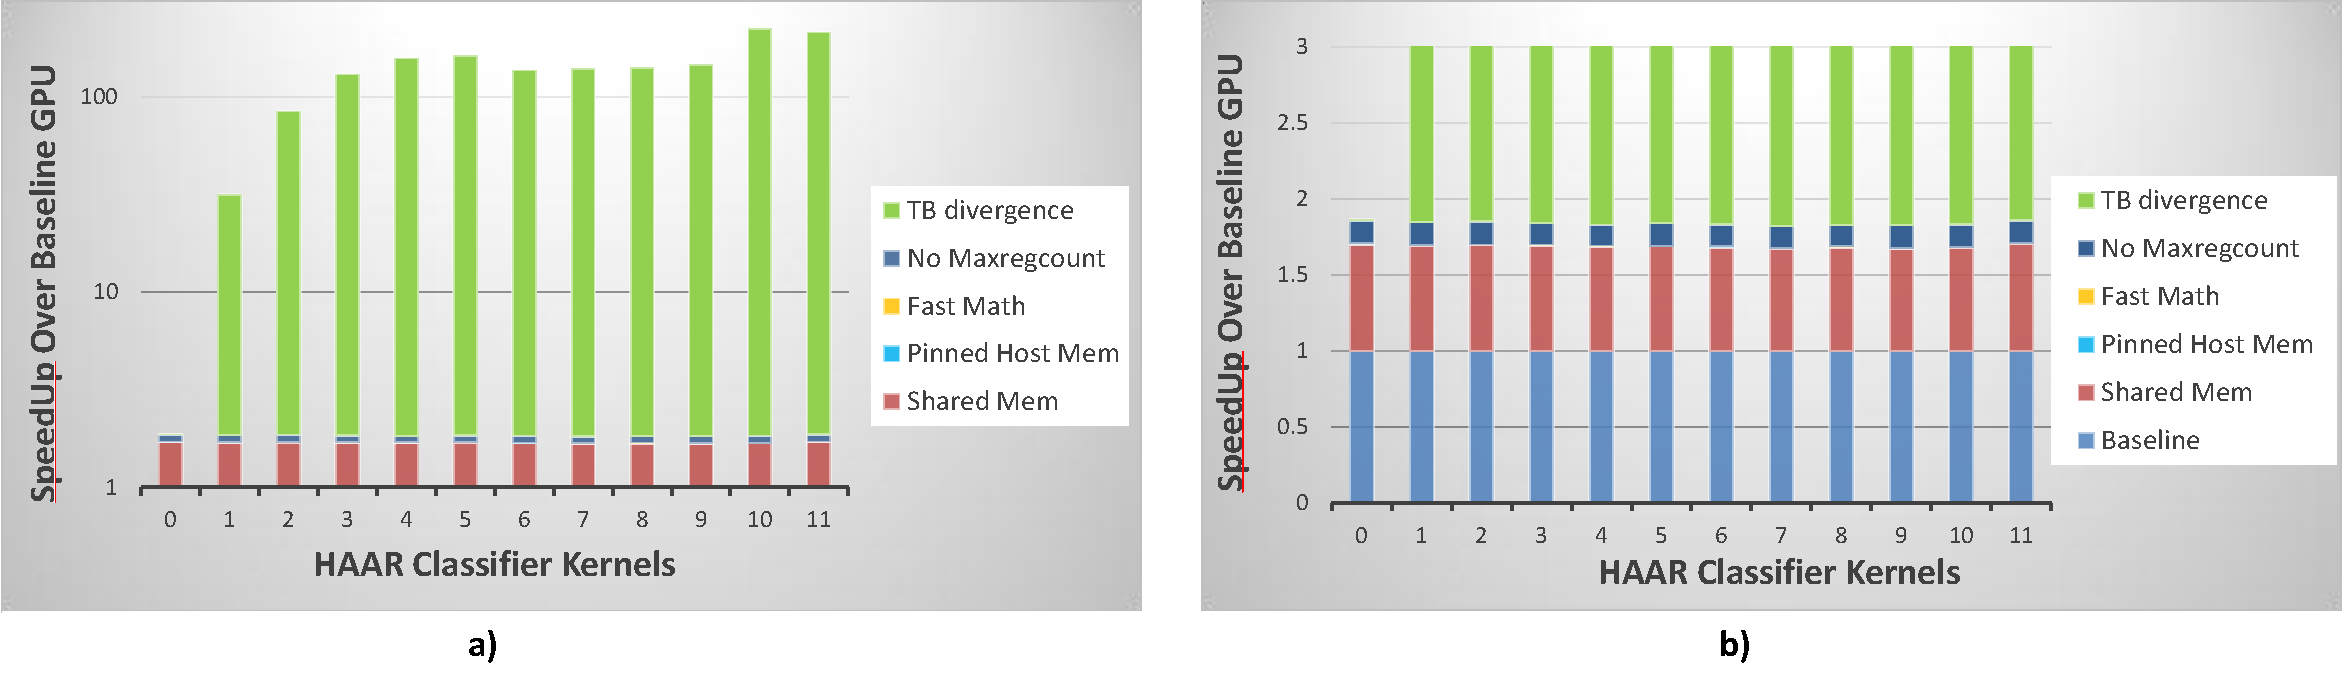
\includegraphics[width=\linewidth]{figs/haar_kernels_crop.pdf}
  \caption{a) HAAR kernels performance; b) Speedup with baseline GPU implementation and magnified version of a)}
  \label{fig:haar_kernels}
\end{figure*}


\begin{figure*}[h]
  \centering
  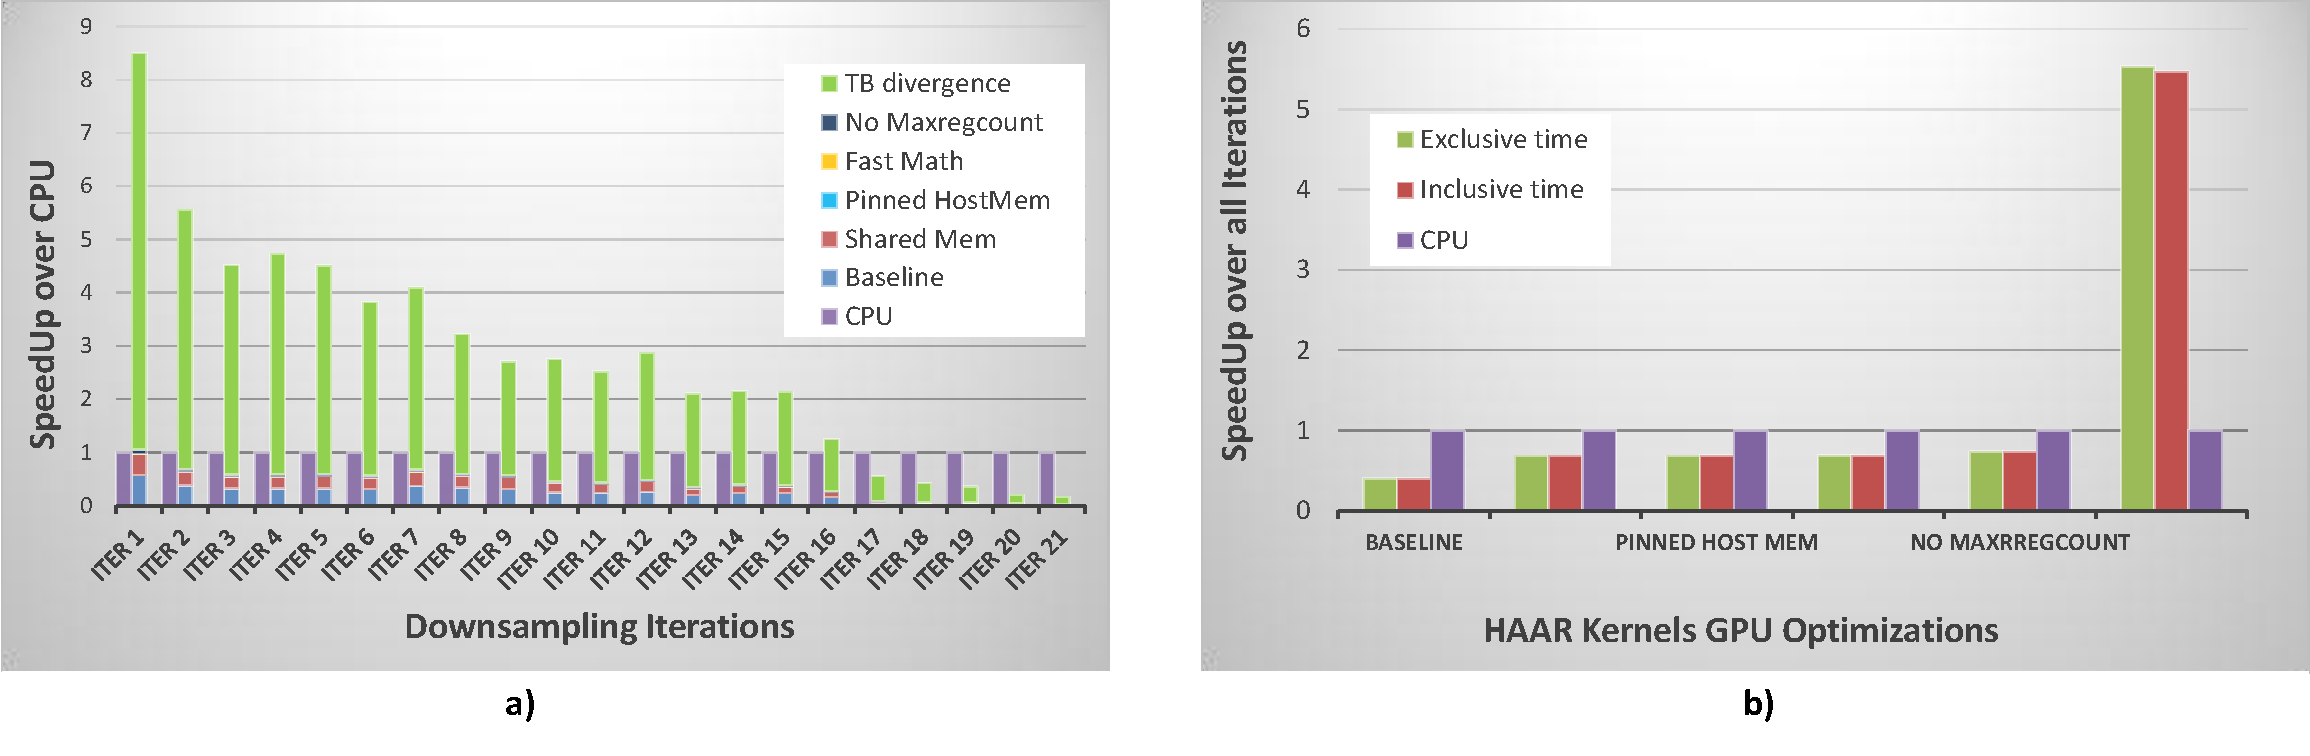
\includegraphics[width=\linewidth]{figs/haar_overall_crop.pdf}
  \caption{a)Performance of HAAR kernels over 21 iterations of 1024 x 1024 image face detection; b) HAAR kernels speedup over CPU for all the iterations}
  \label{fig:haar_overall}
\end{figure*}


\paragraph{}
Figure~\ref{fig:nn_ii_overall} \color{red}{a)} \color{black}{shows} the performance of all 4 NN and II kernels with the optimizations
applied. In overall, we see that \emph{NN + RowScan}, \emph{RowScan} kernels benefit from \emph{extern shared memory} declaration optimization 
and \emph{Transpose 1}, \emph{Transpose 2} kernels take significant benefit from \emph{No bank conflicts} optimization.

Figure~\ref{fig:nn_ii_overall} \color{red}{b)} \color{black}{shows} the combined kernels speedup on GPU over CPU. Here, we just consider the GPU exclusive time as these
kernels don't have any data copying. In overall, we see around \textbf{1.46x} speedup for NN and II kernels over CPU. 
We take the these best performing NN and II kernels for all future evaluations with HAAR classifier kernels.


\subsection{Performance of HAAR Classifier Kernels}
This section overviews the performance of HAAR classifier kernels which
has 97\% of parallelization scope for our face detection implementation.
Figure~\ref{fig:haar_kernels} \color{red}{a)} \color{black}{shows} the performance of 12 HAAR kernels for the image 1024 x 1024 (1 iteration) with optimizations 
detailed in Section~\ref{sec:haar_optim}.
Figure~\ref{fig:haar_kernels} \color{red}{b)} \color{black}{is} the magnified version showing the lower level speedup is detail. The overall speedup of each kernel
is mentioned in the top.
We see that the \emph{shared memory} gives around 1.7x benefit over the baseline GPU implementation. \emph{Pinned host memory} gives almost no benefit
due to the fact that there is very less copying involved in between the kernels. \emph{Fast math} library optimization also gives very negligent performance
as the HAAR kernel involves only 1 \textit{sqrt} function. By removing the maximum registers constraint (\emph{no maxreg} optimization), we get around
1.8x performance benefit over baseline. Finally, the biggest performance boost we get is from the \emph{thread block divergence}, which ranges from 29x to 220x speedup.
Kernel 1 sees no benefit because most of the heavy lifting is done here and it sees no thread block divergence. Whereas, all the other kernels see divergence and get benefited from that.


Figure~\ref{fig:haar_overall} \color{red}{a)} \color{black}{shows} the performance of combined 12 HAAR kernels performance for all the 21 iterations
of the 1024 x 1024 image face detection with all the optimizations explained above. Here, the baseline is CPU and we compare the performance of
all 21 iterations with single threaded performance of CPU. We see similar trend of performance benefit added from the optimizations and we get speedup upto 8.4x
over CPU (this includes the copy time between each kernel). However, it is interesting to see that after iteration 17 GPU has worse performance than the CPU. This is because of the
reason that, from that stages the kernel launch and thread creation overhead if more than the benefit you can get from parallelization. This is an indicator that for smaller images and
when there is low data or thread level parallelism available GPU performs worse than CPU.
Figure~\ref{fig:haar_overall} \color{red}{b)} \color{black}{shows} the combined performance of the entire scanning window stage (12 HAAR kernels with all 21 iterations) with each optimization added. 
We see that thread block divergence gives us the largest benefit of speedup upto \textbf{5.47x} (inclusive time) compared to CPU. We use this optimized kernel for the final face detection speedup comparison.


\subsection{Face Detection Speedup}
We now explain the overall speedup we achieved for the entire face detection algorithm implemented on GPU.
This includes the optimized version of NN + II kernels and optimized version of the HAAR kernel.

\vspace{-0.1in}
\begin{figure}[h]
  \centering
  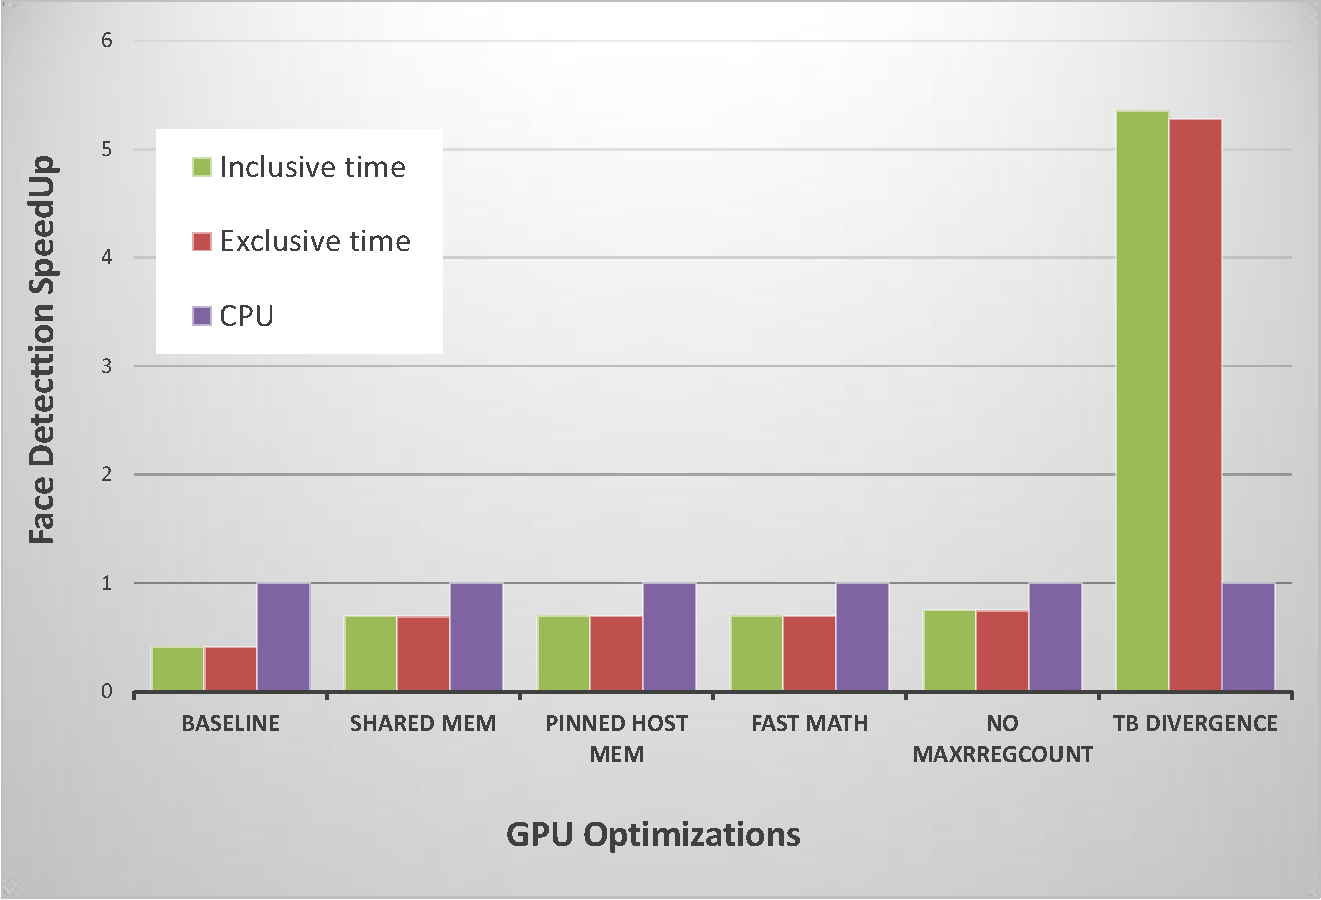
\includegraphics[width=\linewidth]{figs/gpu_overall_crop.pdf}
  \caption{Overall face detection speedup on GPU}
  \label{fig:gpu_overall}
\end{figure}

\vspace{-0.1in}
Figure~\ref{fig:gpu_overall} shows the overall face detection speedup of our implementation 
on GPU. We get a speedup upto \textbf{5.35x} overall over CPU and this includes the inclusive time of copying the
original source image to GPU. We believe this is a good speedup given the amount of serial dependency among HAAR 
classifier kernels. We believe that if parallel scan window processing could be implemented an extra 2-3x speedup can easily be achieved.


\subsection{Scalability and Detection Accuracy}
Figure~\ref{fig:img_sizes} shows GPU face detection speedup over CPU with increasing image sizes. 
As seen in previous results, GPU's parallelization benefit kicks in only after 128 x 128 image size as there
is abundant amount of data and thread level parallelism. As the image size increases GPU easily outperforms CPU and we see
upto 535x speedup with 1024 x 1024 image size. We expect that the speedup increases linearly as we scale up the image.



\begin{figure}[h]
  \centering
  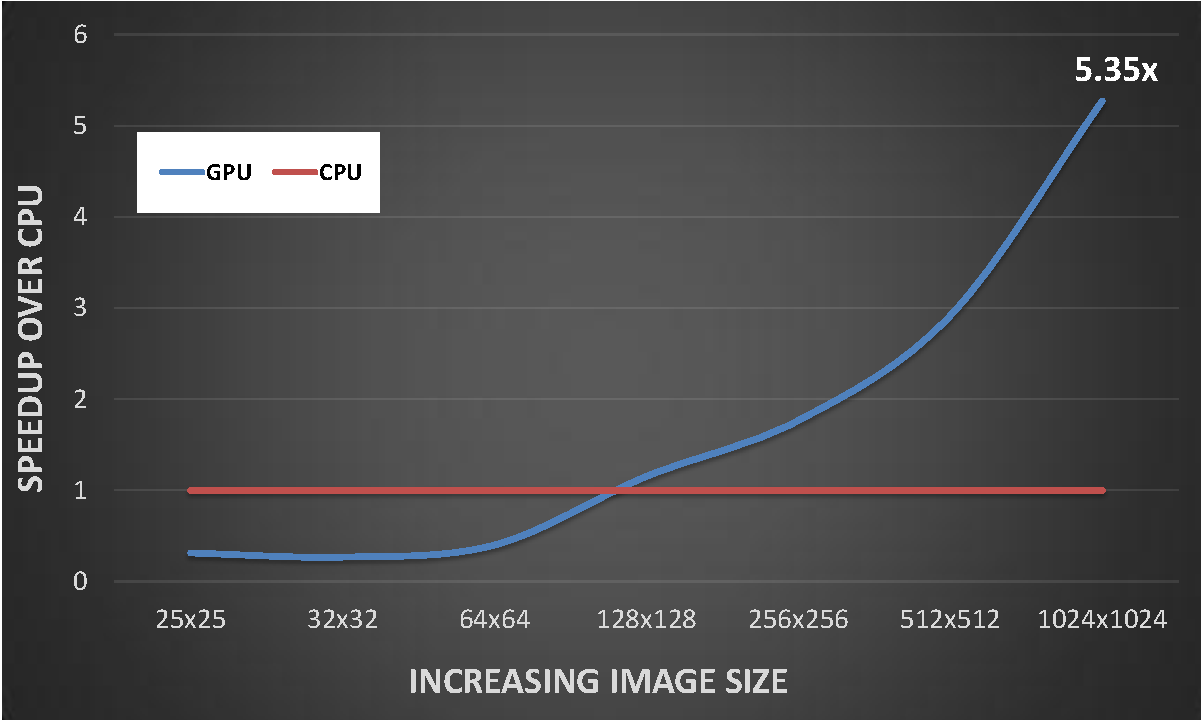
\includegraphics[width=\linewidth]{figs/image_size_crop.pdf}
  \caption{GPU speedup with varying image sizes}
  \vspace{0.05in}
  \label{fig:img_sizes}
\end{figure}

\begin{table}[]
    \centering
    \scalebox{0.65}{
        \begin{tabular}{|c|c|c|c|c|c|l|c|}
        \hline
        \textbf{Number of Faces}     & \textit{1} & \textit{2} & \textit{4} & \textit{8} & \textit{16} & 32    & \textit{Average Detection Rate (\%)} \\ \hline
        \textbf{Detection Rate (\%)} & 100        & 100        & 100        & 87.5       & 100         & 93.75 & \textbf{96.875}                      \\ \hline
        \end{tabular}
        }
        \vspace{0.1in}
        \caption{Face Detection Accuracy on GPU}
        \label{table:acur}
\end{table}


We also performed a small experiment of the algorithm accuracy. Although this is an algorithmic perspective
and not the implementation outcome, we  wanted to see how well the Viola Jones algorithm performs on GPU in detecting faces. 
Table~\ref{table:acur} shows the detection accuracy for different number of faces in the image. With random selection of images and
number of faces, we see upto 96.875\% accuracy in detecting faces. Figure~\ref{fig:detect} shows some example faces detected and as the accuracy test
confirm, one of the faces did not get detected in the test. This could be because of tilted face, or some of the features not present in the classifier filters.
But still given the simple classifier information, face detection can be easily be extended on GPU for better speedups and with more robust face detection algorithms
we expect to get better speedups and detection rate. 

\begin{figure}[h]
  \centering
  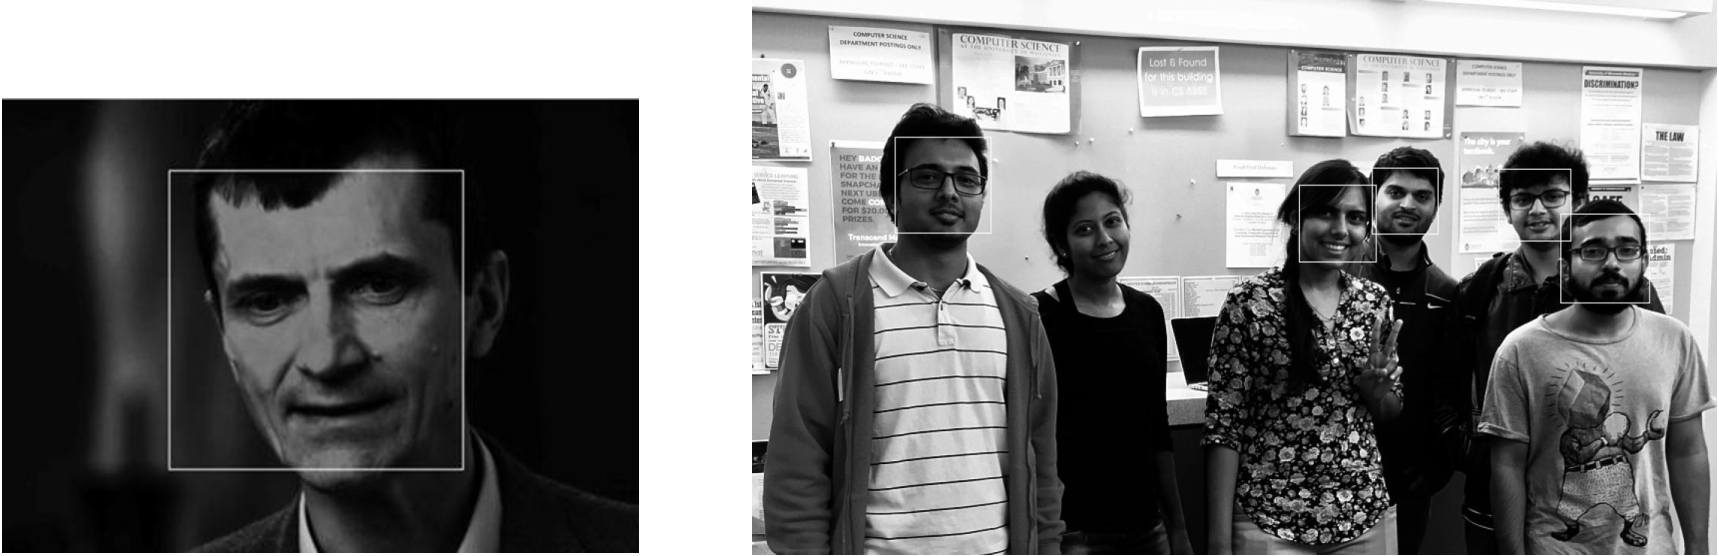
\includegraphics[width=\linewidth]{figs/face_detected_crop.pdf}
  \caption{Examples of faces detected on GPU}
  \label{fig:detect}
\end{figure}



